% Plan 
% 
% Wed
% - [x] change position normalization of existing code to [0, 1)
% - [x] grid points
% Thu
% - [x] nearest grid point weighting
%   - [ ] write-up
% - [x] linear weighting
%   - [ ] write-up
% Fri
% - [x] Poisson solver
%   - [x] boundary conditions
%   - [x] finite diff matrix
%   - [x] solve
%   - [ ] write-up
% Sat
% - [ ] normalization for poisson solver
% - [x] charge background
% - [x] initialization step
%   - [ ] write-up
% - [x] particle push
%   - [ ] write-up
% - [ ] field energy diagnostic
% - [ ] stationary two-electron test case
%   - [ ] set up problem and find oscillations
%   - [ ] determine oscillation frequency
%   - [ ] find theoretical frequency
%   - [ ] compare theoretical freq for 0th and 1st order
%   - [ ] write-up
% Sun
% - [ ] moving two-electron test case
%   - [ ] setup particle velocities and run
%   - [ ] find simple harmonic motion and determine freq
%   - [ ] find theoretical freq
%   - [ ] compare theoretical freq for 0th and 1st order
%   - [ ] find velocity that lets paths cross
%   - [ ] write-up
% Mon/Tue
% - [ ] cold static particles
%   - [.] initialize system and velocity perturbation
%   - [.] measure energy frequency
%   - [ ] vary plasma freq
%   - [ ] phase error
%   - [ ] write-up
% Wed
% - [ ] write conclusions
\documentclass[%
 reprint,
%superscriptaddress,
%groupedaddress,
%unsortedaddress,
%runinaddress,
%frontmatterverbose, 
%preprint,
%preprintnumbers,
%nofootinbib,
%nobibnotes,
%bibnotes,
 amsmath,amssymb,
 aps,
%pra,
%prb,
%rmp,
%prstab,
%prstper,
%floatfix,
]{revtex4-2}

\usepackage{graphicx}% Include figure files
\usepackage{dcolumn}% Align table columns on decimal point
\usepackage{bm}% bold math
\usepackage{physics}
%\usepackage{hyperref}% add hypertext capabilities
%\usepackage[mathlines]{lineno}% Enable numbering of text and display math
%\linenumbers\relax % Commence numbering lines

%\usepackage[showframe,%Uncomment any one of the following lines to test 
%%scale=0.7, marginratio={1:1, 2:3}, ignoreall,% default settings
%%text={7in,10in},centering,
%%margin=1.5in,
%%total={6.5in,8.75in}, top=1.2in, left=0.9in, includefoot,
%%height=10in,a5paper,hmargin={3cm,0.8in},
%]{geometry}

\begin{document}

\preprint{APS/123-QED}

\title{An Electrostatic Vlasov-Poisson Particle-in-Cell Model}% Force line breaks with \\

\author{Evan Bluhm}
%  \altaffiliation[Also at ]{Physics Department, XYZ University.}%Lines break automatically or can be forced with \\
% \author{Second Author}%
%  \email{Second.Author@institution.edu}
% \affiliation{%
%  Authors' institution and/or address\\
%  This line break forced with \textbackslash\textbackslash
% }%

% \collaboration{MUSO Collaboration}%\noaffiliation

% \author{Charlie Author}
%  \homepage{http://www.Second.institution.edu/~Charlie.Author}
% \affiliation{
%  Second institution and/or address\\
%  This line break forced% with \\
% }%
% \affiliation{
%  Third institution, the second for Charlie Author
% }%
% \author{Delta Author}
% \affiliation{%
%  Authors' institution and/or address\\
%  This line break forced with \textbackslash\textbackslash
% }%

% \collaboration{CLEO Collaboration}%\noaffiliation

\date{April 21, 2021}% It is always \today, today,
             %  but any date may be explicitly specified
% \begin{abstract}

% abstract go here

% % \begin{description}
% % \item[Usage]
% % Secondary publications and information retrieval purposes.
% % \item[Structure]
% % You may use the \texttt{description} environment to structure your abstract;
% % use the optional argument of the \verb+\item+ command to give the category of each item. 
% % \end{description}
% \end{abstract}

%\keywords{Suggested keywords}%Use showkeys class option if keyword
                              %display desired
\maketitle

%\tableofcontents


\section{Electrostatic Particle-In-Cell}

In our previous project, we laid the groundwork for a one-dimensional particle in cell (PIC) integrator, implemented in Python. Now, we will introduce the long range electrostatic force to complete a collision-less electrostatic PIC solver. Even in this very simple model, we are able to demonstrate bulk plasma phenomena such as Langmuir oscillations, as well as investigate the stability and accuracy of the numerical integration scheme.

The governing equations for our electrostatic PIC model for each particle $i$ are:

\begin{eqnarray}
\dv{\vec v_i}{t} & =  & \left( \frac{q_i}{m_i} \right) \vec E\\
\dv{\vec r_i}{t} & = & \vec v_i
\end{eqnarray}

where $\vec E$ and $\vec B$ are the electromagnetic fields computed at the closest spatial grid location to particle $i$. To integrate position and velocity forward in time by discrete steps $\Delta t$, we use a leapfrog integration scheme. Position and velocity are separated in time by ($\Delta t/2$), so that the average value of $\vec x$ over the step is used to calculate $\Delta \vec v$, and vice-versa. At each time step, we calculate the electric field $\vec E$ from the position $\vec x$, as described in the following section.

\begin{eqnarray}
\frac{{x_i}^{n+1} - {x_i}^n}{\Delta t} = {v_i} ^{n + 1/2} \label{push}
\end{eqnarray}
\begin{eqnarray}
\frac{{v_i} ^{n+1/2} - {v_i}^{n - 1/2}}{\Delta t} = \frac{q_i}{m_i} E_i ^n \label{accel}
\end{eqnarray}

This leapfrog integration scheme is a symplectic integrator (it preserves the Hamiltonian structure of each time step), and so conserves energy stepping either forward or backwards in time. It has second-order accuracy, and as we shall see later, it is stable if $\omega_0 \Delta t < 2$.

\section{Normalization}

The values which the PIC solver operates on are not in SI units. Rather, most quantities have been normalized such that the scales of interest are of order unity. The plasma frequency $\omega_p$, the electric constant $\epsilon_0$, and the charge-to-mass ratio of the particles $q/m$ are inputs to the program. These determine the time, mass, and charge scales reported by the program. By default, $\omega_p = 1$, $\epsilon_0 = 1$, and $q/m = -1$. The initial positions and velocities of the particles determine the units of length. Within the program, the charge $q$ and mass $m$ of each particle are calculated from the input parameters as:

\begin{equation}
q = \frac{\omega_p ^2 (L/N) \epsilon_0}{q/m} \qquad m = \frac{q}{(q/m)}
\end{equation}

Here, $N$ is the number of particles and $L$ is the length scale of the system. This normalization results in quantities that are easy to compare and visualize at similar absolute scales. The units of time are $1/\omega_p$, making it straightforward to run the integrator for a certain number of plasma oscillations by setting the \texttt{t\_max} parameter. It is possible to further normalize the computed quantities by combinations of $\Delta t$ and $\Delta x$ to avoid unnecessary repeated multiplication, but this implementation has chosen not to do so for ease of plotting and interpretation of the raw results.

\section{Particle Weighting}

In the PIC method, we treat particles as having a finite extent, rather than point particles. The forces acting on the particles are those of the long-range electromagnetic fields, which we compute at a finite set of points on a uniform grid. This method resolves the issue of treating $N$ singularities in the Coulomb force, and absolves us of the need to compute $N^2$ particle-particle interactions. Particles are assigned as source terms to the grid by a ``weighting'' function. Once fields on the grid have been computed, the force on each particle is assigned in turn by a similar weighting process.

Within \texttt{weighting.py}, two different weighting functions for particles and fields have been implemented. The first weighting is the zeroth-order ``nearest grid point'' method. When weighting particles to the grid, each particle simply contributes its charge to the nearest grid point, and likewise when computing the force on a particle we simply use the value of the field at the nearest grid point. This is computationally the fastest weighting method, but introduces noise as particles seem to jump instantaneously from one grid point to the next.

The second weighting method is a first-order linear interpolation between the two nearest grid points. At the cost of some extra cycles, we get much smoother charge density and fields. For a particle at position $x_i$ with charge $q_i$, we distribute its charge to $x_j$ and $x_{j+1}$, the two nearest points on the grid, respecting the periodic boundary conditions:

\begin{equation}
\rho_j = q_i \frac{x_{j+1} - x_i}{\Delta x} \qquad \rho_{j+1} = q_i \frac{x_i - x_j}{\Delta x}
\end{equation}

The first-order field weighting performs the same linear interpolation, but in the opposite direction. The field  at position $x_i$ is calculated as:

\begin{equation}
E(x_i) = \frac{x_{j+1} - x_i}{\Delta x} E_j + \frac{x_i - x_j}{\Delta x} E_{j + 1}
\end{equation}

The weighting order used within the program is determined by the \texttt{weighting\_order} input parameter.

\section{Field Solver}

At each time step, we solve for the forces on all particles by estimating the electric field at each particle's location. Rather than directly computing the electrostatic interactions between all particles using Coulomb's law, it is far easier to solve Poisson's equation for the electric scalar potential $\phi$, and calculate its gradient:

\begin{eqnarray}
\nabla ^2 \phi & = & - \rho_c / \epsilon_0 \\
\vec E & = & - \grad \phi
\end{eqnarray}

where $\rho_c$ is the charge density. Weighting the particles to the grid gives $\rho_j$. For meaningful results, the overall charge density of the system must be zero, so a constant background of opposite charge is added to $\rho_j$ to enforce charge neutrality. We also absorb the $\epsilon_0$ normalization into $\rho_j$. The program uses a finite difference method to solve Poisson's equation for $\phi_j$, and to compute $E_j$. The finite difference operators used are:

\begin{eqnarray}
\frac{\phi^n _{j+1} - 2 \phi_j ^n + \phi^n_{j-1}}{\Delta x ^2} = - \rho _j ^n \\
E_j ^n = - \frac{\phi ^n _{j+1} - \phi ^n _{j-1}}{2 \Delta x}
\end{eqnarray}

Poisson's equation in this finite difference form can be expressed as a matrix equation $\vec A \vec \phi = \vec \rho $. Solving for $\vec \phi$ is as simple as inverting $\vec A$. For our system with periodic boundary conditions, however, the solution $\vec \phi$ is lacking a gauge and, with the result that $\vec A$ is singular. In the program, we resolve the gauge ambiguity by setting $\phi_0 = 0$, and disregard the value of $\rho_0$ as it is redundant. We can write the resulting matrix equation in the following form:

\begin{equation}
\frac{1}{\Delta x ^2}\begin{bmatrix}
1 & 0 & 0 & 0 & \ldots & 0 \\
1 & -2 & 1 & 0 & \ldots & 0 \\
0 & 1 & -2 & 1 & \ldots & 0 \\
 & \ldots & \ldots & \ldots &  & 0 \\
0 & \ldots & 1 & -2 & 1 & 0 \\
0 & \ldots & 0 & 1 & -2 & 1 \\
-1 & \ldots & 0 & 0 & 1 & -2 \\
\end{bmatrix} \begin{bmatrix}
\phi_0 \\ \phi_1 \\ \phi_2 \\ \phi_j \\ \phi_{m-3} \\ \phi_{m-2} \\ \phi_{m-1} 
\end{bmatrix} = \begin{bmatrix}
0 \\ \rho_1 \\ \rho_2 \\ \rho_j \\ \rho_{m-3} \\ \rho_{m-2} \\ \rho_{m-1} 
\end{bmatrix}
\end{equation}

With the symmetry broken, this matrix is invertible. The inverted $\vec A^{-1}$ is constant throughout the time integration, and is only computed once at the beginning of the run. The functions to compute both $\vec A^{-1}$ and $E_j$ are included in the \texttt{poisson.py} module. A set of associated \texttt{pytest} test cases use constructed solutions to validate that the finite difference method is accurate to the expected $O(\Delta x ^2)$.

\section{Initialization}

The initial conditions provided to each run of the program are the positions and velocities at $t=0$, $x_i ^0$ and $v_i ^0$. As with any time-centered method, we require a single iteration of a backwards integrator to find $v_i ^{-1/2}$. In the \texttt{initialize()} routine, the fields $E_j ^0$ are calculated from $x_i ^0$ and used for a half Euler step backwards:

\begin{equation}
v _i ^{-1/2} = v_i ^0 - \frac{\Delta t}{2} \frac{q_i}{m_i} E_i ^n
\end{equation}

\section{Particle Push}

With $E_j$ in hand, we can accelerate the particles from $v^{n - 1/2}$ to $v^{n + 1/2}$ following equation \eqref{accel}. It is convenient to compute the kinetic energy diagnostic at the same time, as described in Birdsall, so that the resulting kinetic energy is centered at time $n$ along with the fields:

\begin{equation}
KE^n = \sum_i \frac{1}{2} m_i (v_i ^{n - 1/2}) (v_i ^{n + 1/2})
\end{equation}

With $v^{n + 1/2}$ we can move $x^n$ to $x^{n+1}$ using equation \ref{push}. Finally, if particles have moved outside the periodic system, they are shifted accordingly.

\section{Input Parameters}

The conditions for each run are specified as global variables in a configuration file, loaded when \texttt{pic1.py} is run. The configurable parameters are the following:

\begin{itemize}
    \item \texttt{N}: The number of particles.
    \item \texttt{M}: The number grid cells.
    \item \texttt{initial\_x}: An array of initial particle positions.
    \item \texttt{initial\_v}: An array of initial particle velocities.
    \item \texttt{wp}: The plasma frequency $\omega_p$.
    \item \texttt{qm}: The charge-to-mass ratio of the particles.
    \item \texttt{eps0}: The normalization of $\epsilon_0$.
    \item \texttt{dt}: The time step $\Delta t$.
    \item \texttt{t\_max}: The run integrate forward by $t_{max} / \Delta t$ iterations.
    \item \texttt{weighting\_order}: The order of the weighting functions used, either 0 or 1.
\end{itemize}

The run conditions described in the following sections are provided in several configuration files. The provided file \texttt{config\_langmuir\_displacement.py} initializes two stationary particles and visualizes the resulting simple harmonic motion. The file \texttt{config\_langmuir\_moving.py} is very similar, but here the particles have an initial velocity. The file  \texttt{config\_leapfrog\_instability.py} initializes a cold, uniform distribution with a small periodic velocity perturbation in order to investigate the leapfrog instability.

\section{Langmuir Oscillations}

\begin{figure}
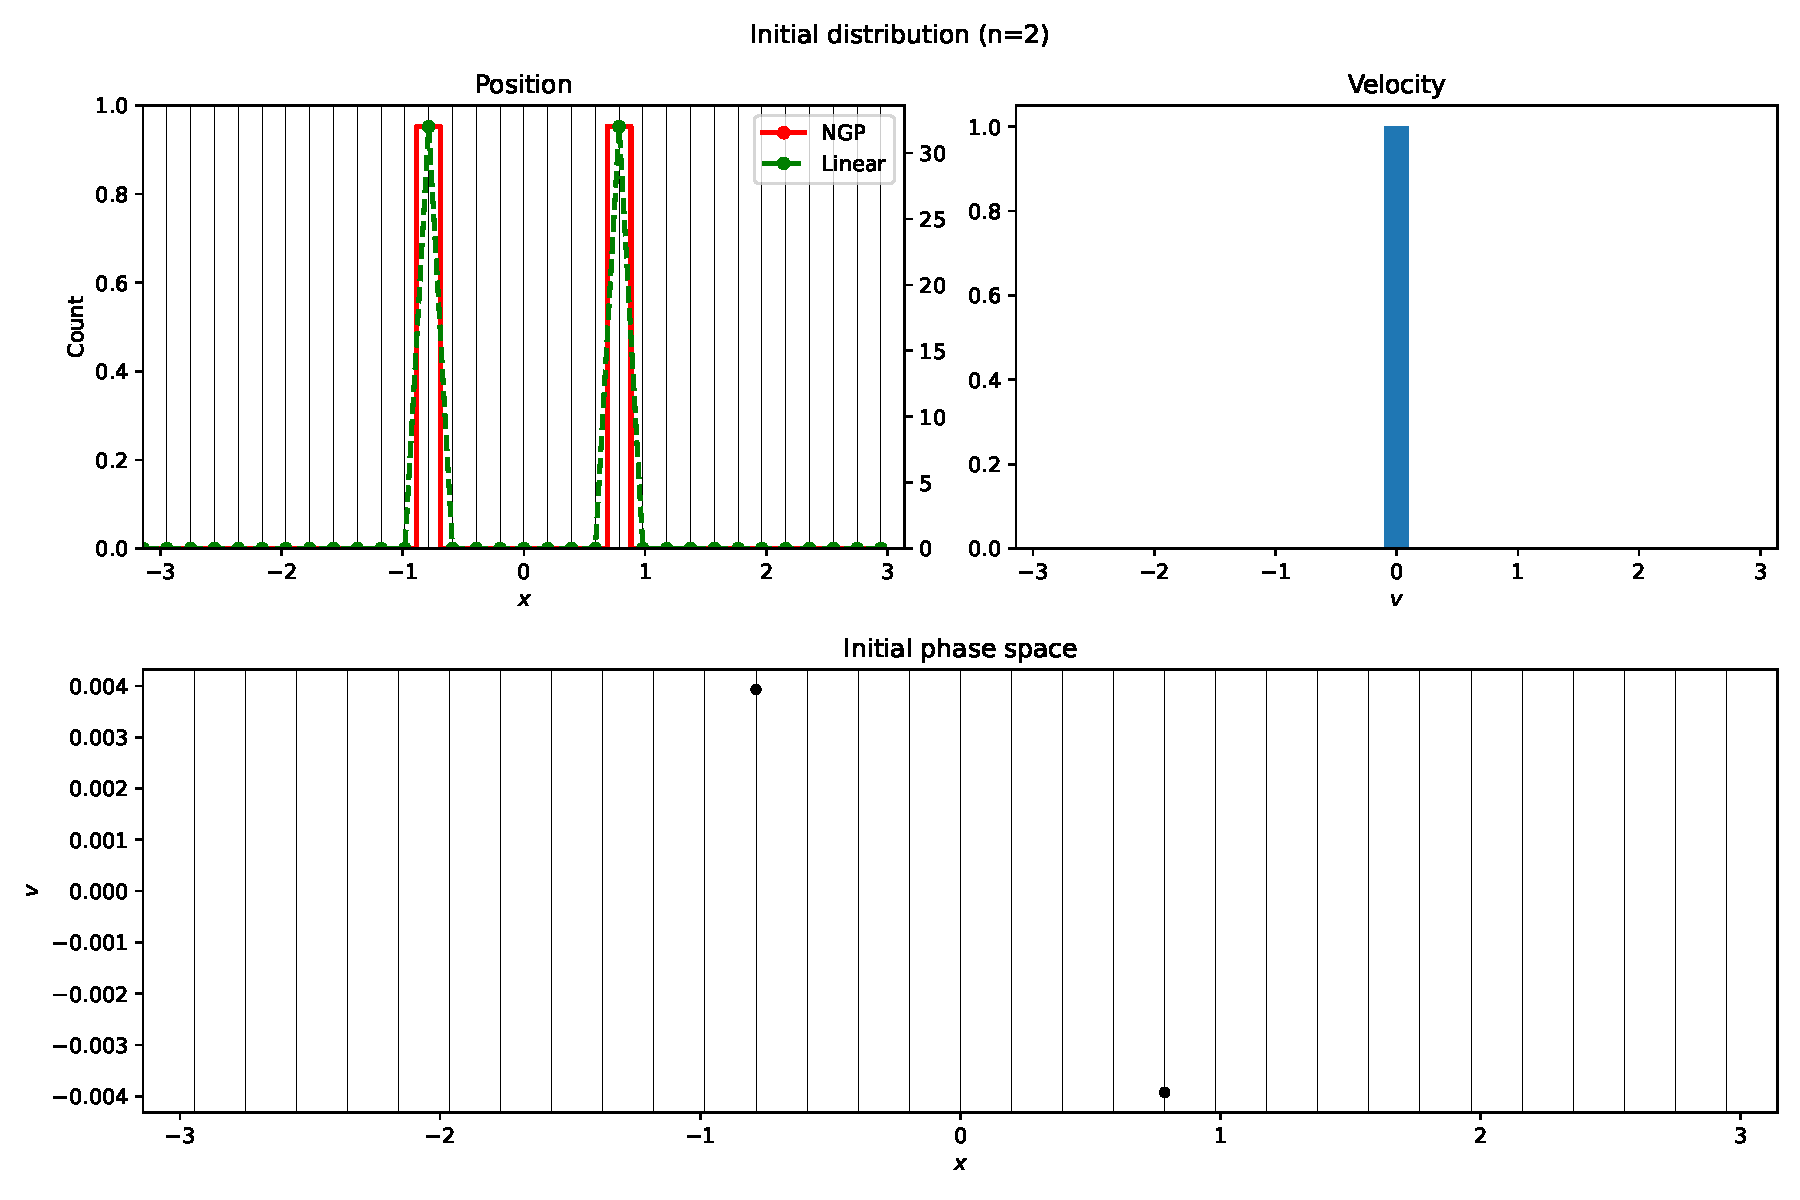
\includegraphics[width=0.9\linewidth]{proj2/langmuir_stationary_init.pdf}
\caption{\label{fig:two-particle-stationary}Initial run conditions for simple harmonic motion. Vertical lines denote the grid points. The nearest grid point weighting is visualized as a red step function, and the linear weighting is shown in dashed lines. The initial backwards half-step has already been applied to $v^0$, as shown.}
\end{figure}

\begin{figure}
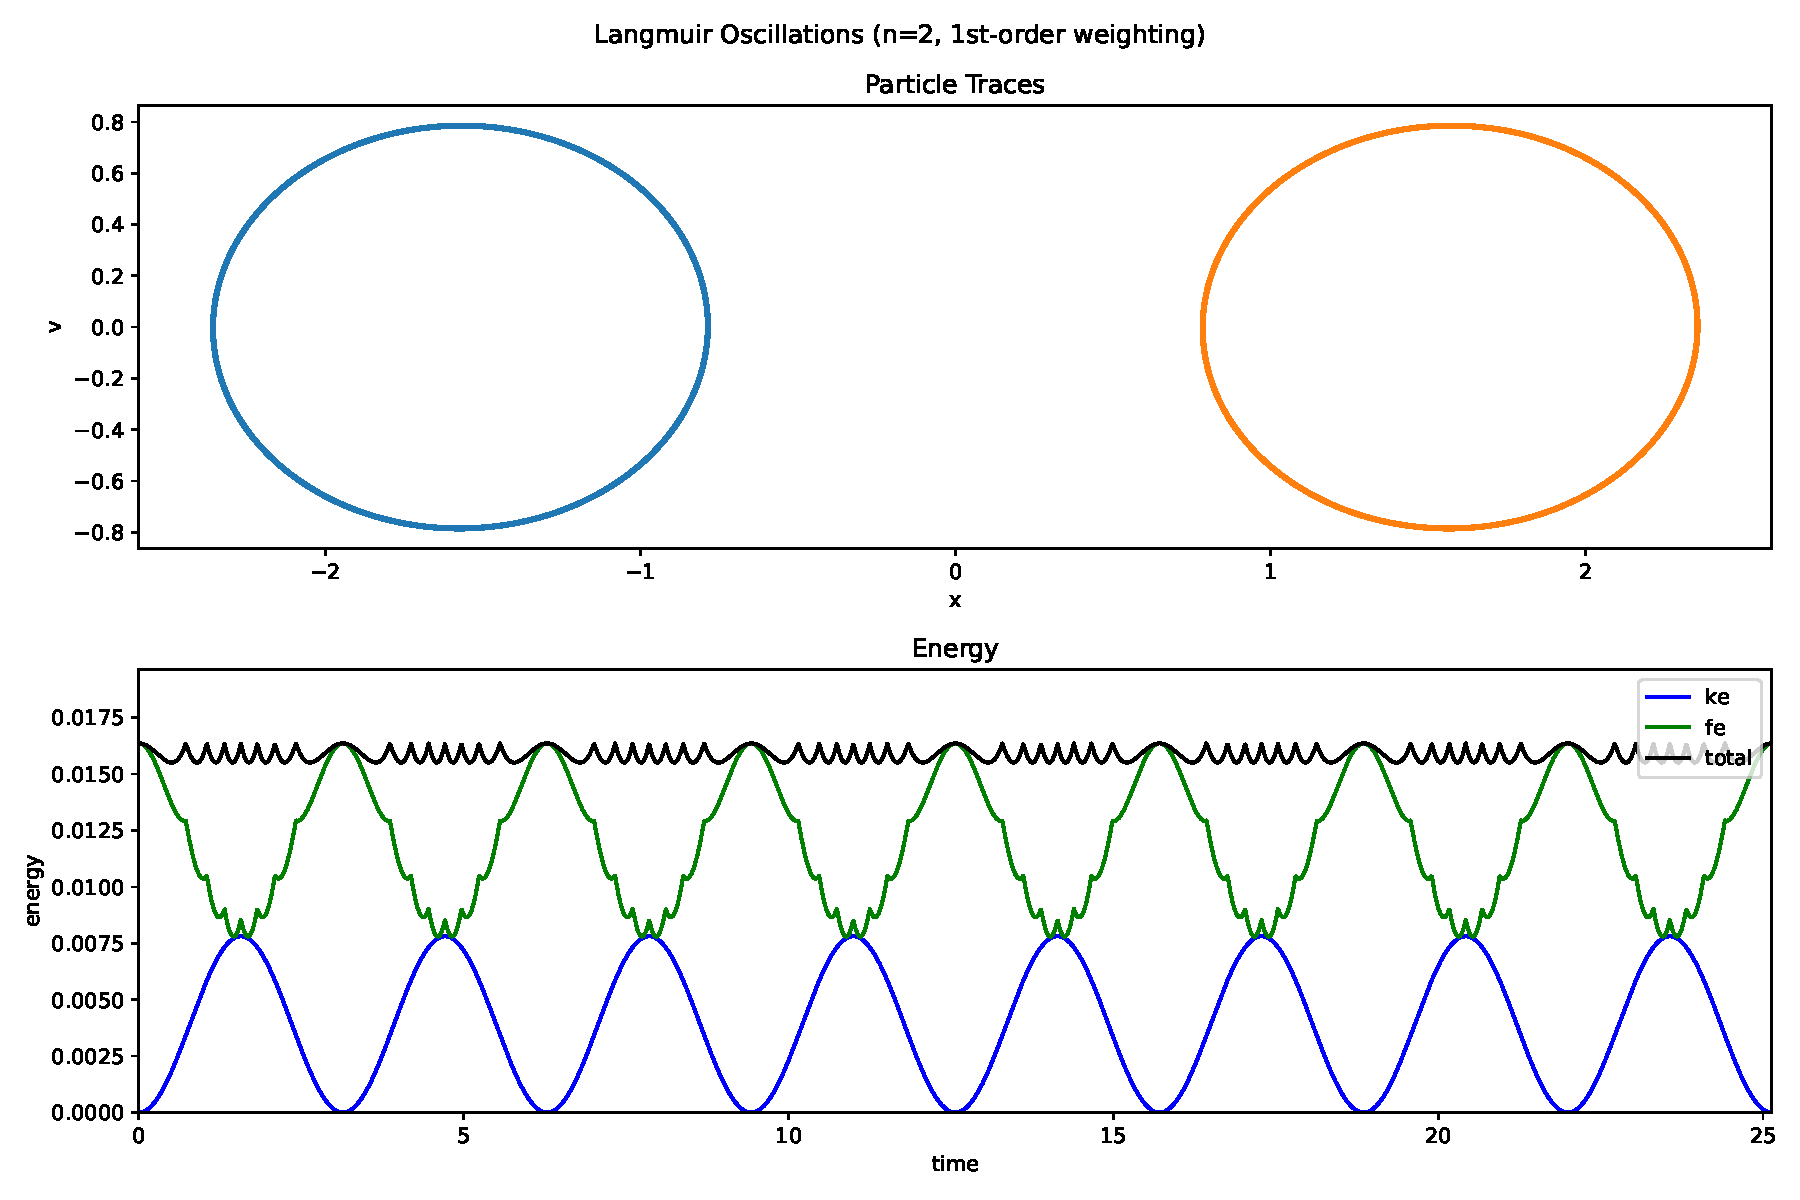
\includegraphics[width=0.9\linewidth]{proj2/langmuir_stationary_trace.pdf}
\caption{\label{fig:two-particle-stationary-trace}Traces of the two stationary particles in phase space. The total kinetic energy and total field energy are plotted in time, revealing the fundamental frequency of the system. First-order weighting functions were used. Run parameters were $M=32$, $\omega_p=1$, $\Delta t = 0.01$, and $t_{max} = 8 \pi$}
\end{figure}

The first configuration of interest is shown in Figure \ref{fig:two-particle-stationary}. Two stationary particles are placed near each other and allowed to undergo simple harmonic motion. The resulting behavior is shown in Figure \ref{fig:two-particle-stationary-trace}. The simple harmonic oscillation is very clear in the particle traces. Since the energy terms are squared quantities, the kinetic and field energies repeat at double the oscillation frequency. Over the course of the $t_{max} = 8 \pi$ run, there are 4 clear oscillatory periods, giving $2 \pi \omega = \frac{8 \pi}{4}$, which is the expected $\omega = 1 = \omega_p$.

We can make a more accurate measurement of $\omega$ by allowing the program to iterate over many oscillatory periods and counting the number of times each particle crosses back through the same region, as implemented in \texttt{count\_crossings()}. Setting $t_{max}$ to $200 \pi / \omega_p$, we still find $\omega = 1.0$ for first-order weighting, but $\omega = 1.0075$ for zeroth-order weighting. The non-physical dispersive effects of the zeroth-order particle weighting on a finite grid become even more apparent as we increase the grid spacing $\delta x$.

The second configuration we consider is identical to the first, except the particles are initialized with twice the separation and an initial velocity $v_0$. Their initial locations in phase space are $(- \pi / 2, v_0)$ and $(\pi / 2, v_0)$. For $v_0 = 0$, the symmetric system remains stationary. For $v_0 < \pi/2$, with first-order weighting we see simple harmonic oscillation with frequency $\omega_0$, regardless of the value of $v_0$, as shown in Figure \ref{fig:two-particle-moving-trace}. With nearest grid point weighting, for very small values of $v_0/\Delta x$ we again observe noisy deviations from $\omega = \omega_p$. As we increase $v_0$ beyond $\pi/2$, the particles overcome their Coulomb barrier and switch places. The resulting motion is no longer simple harmonic, and the frequency of oscillations grows with increasing $v_0$ as shown in Figure \ref{fig:two-particle-moving-dispersion}.

\begin{figure}
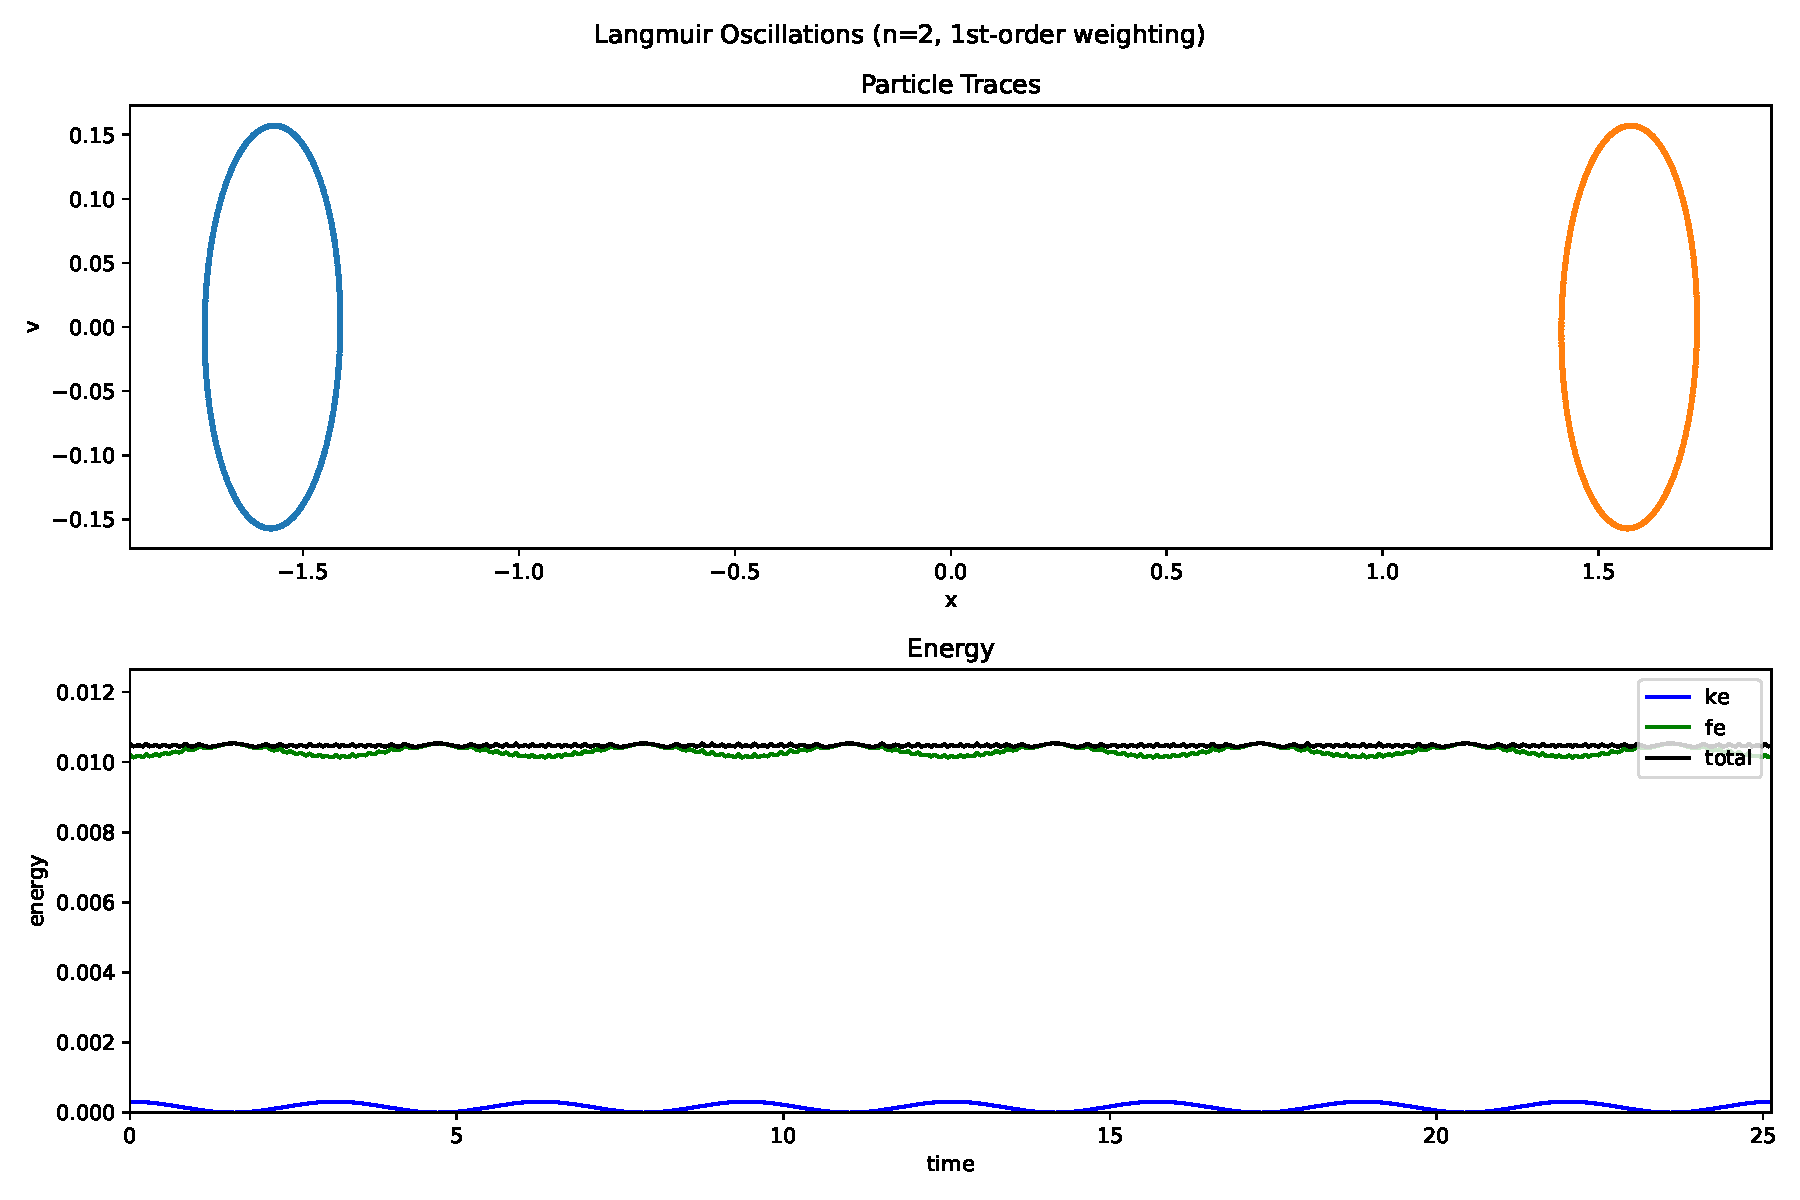
\includegraphics[width=0.9\linewidth]{proj2/langmuir_moving_trace.pdf}
\caption{\label{fig:two-particle-moving-trace}Traces of two particles initialized with a small velocity towards each other. $v_0 = \pi / 20$. The frequency of oscillations remains $\omega = \omega_p$, regardless of $v_0$.}
\end{figure}

\begin{figure}
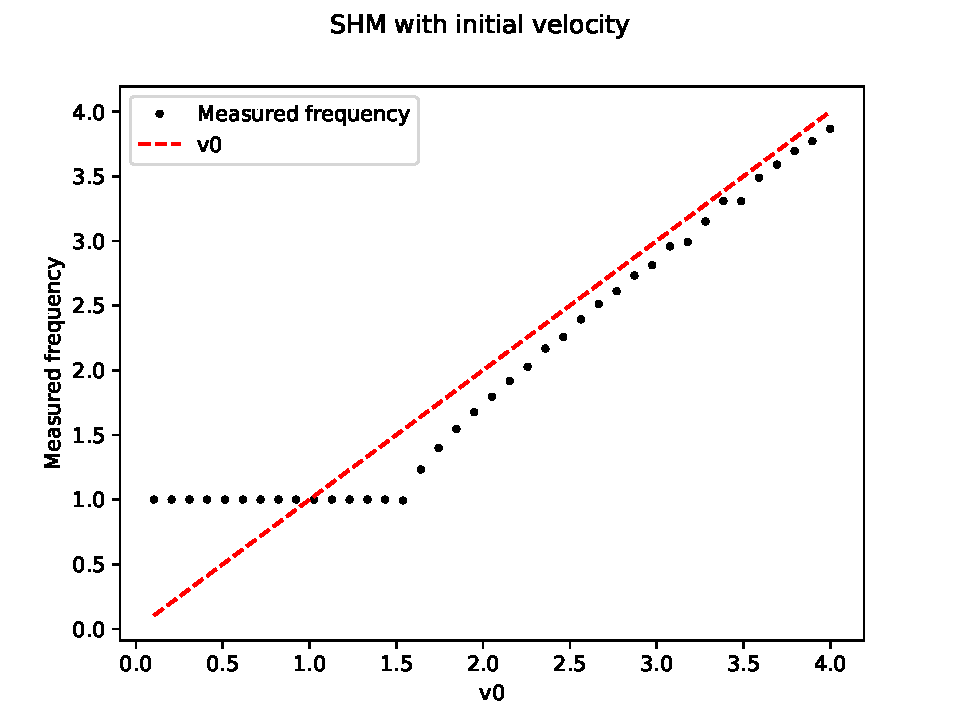
\includegraphics[width=0.9\linewidth]{proj2/coupled_oscillators_dispersion.pdf}
\caption{\label{fig:two-particle-moving-dispersion}Dispersion relation for two coupled oscillators separated by distance $\pi$ with an initial velocity $v_0$. For $v_0 < \pi / 2$, the frequency of oscillations is independent of $v_0$. For $v_0 > \pi / 2$, the frequency grows with $v_0$.}
\end{figure}

\section{Leapfrog Instability}

The final configuration of interest is shown in Figure \ref{fig:leapfrog-init}. A cold, static plasma is given a small periodic velocity perturbation. Because the plasma is nearly uniform, the finite difference equations \eqref{push} and \eqref{accel} become homogeneous:

\begin{figure}[h]
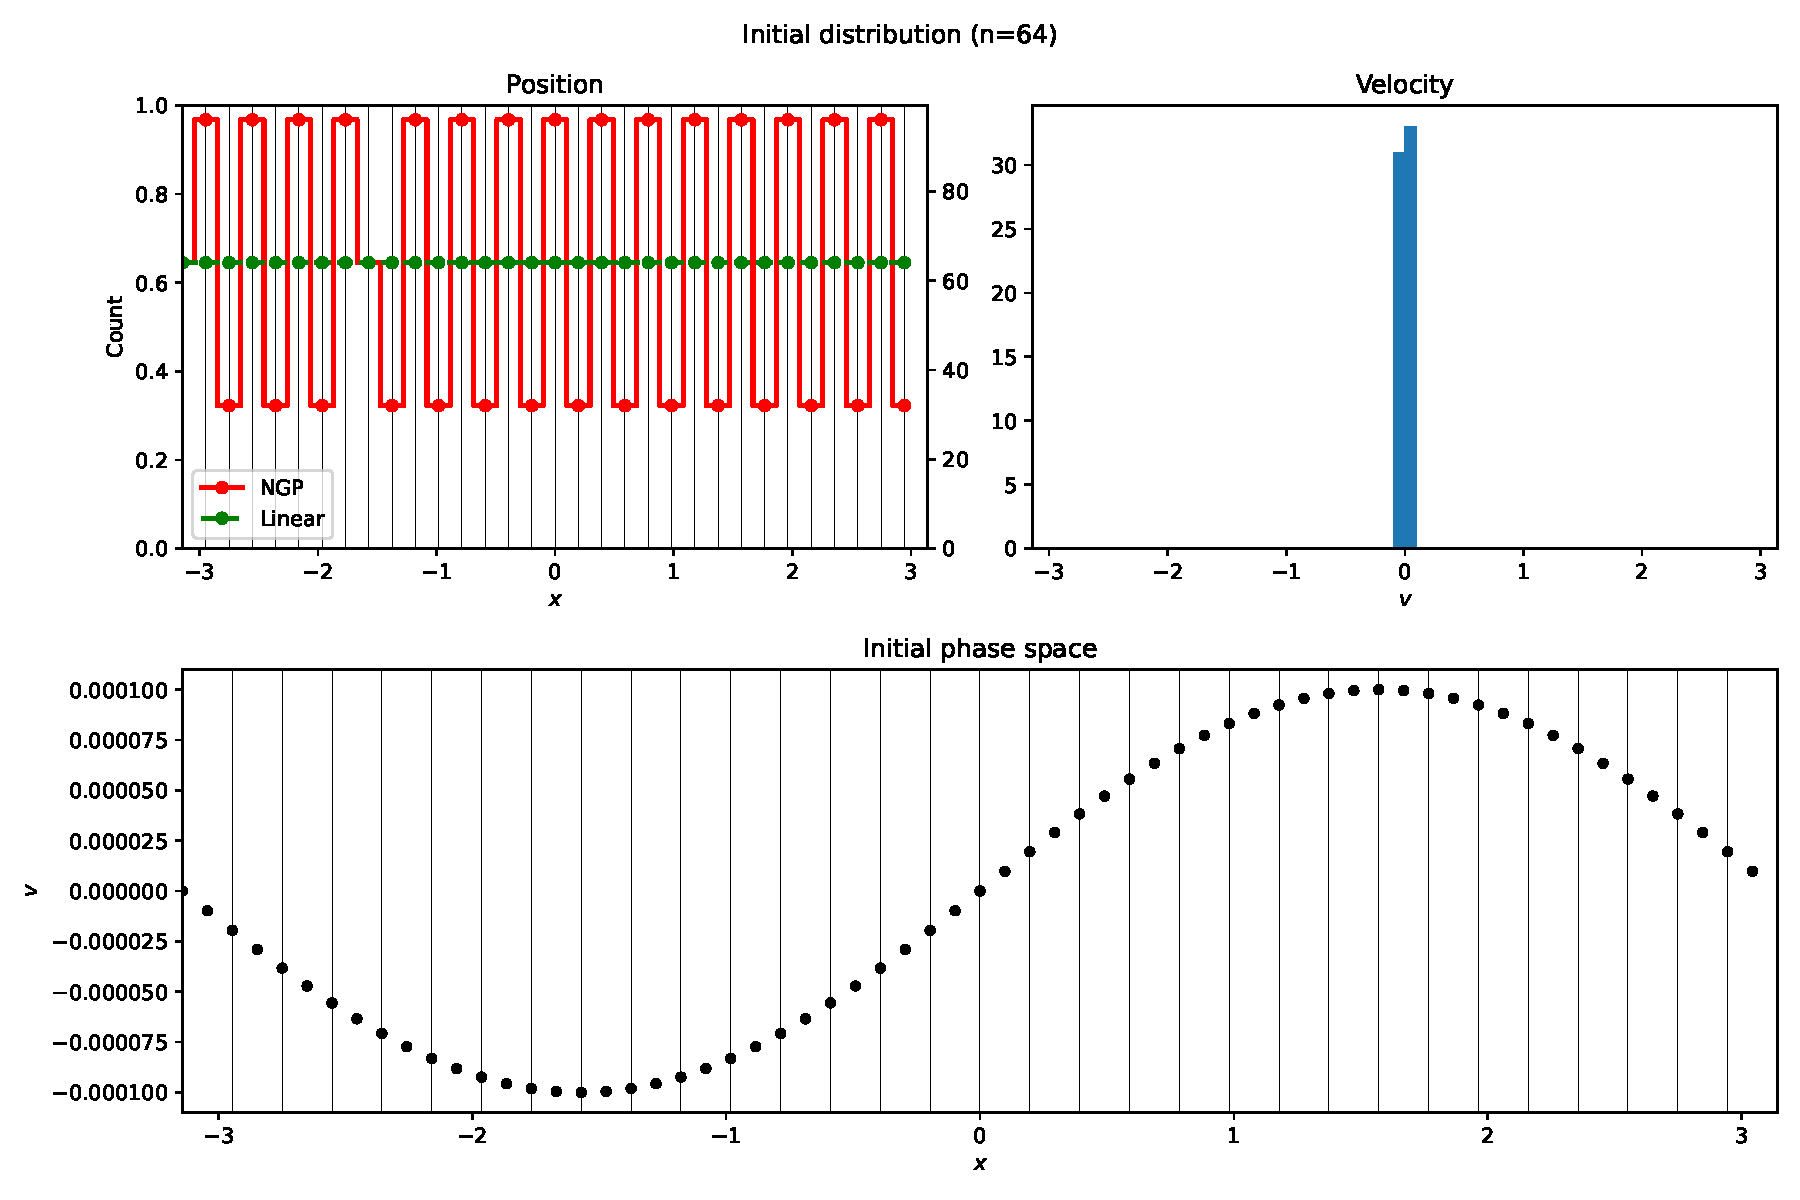
\includegraphics[width=0.9\linewidth]{proj2/leapfrog-instability-setup.pdf}
\caption{\label{fig:leapfrog-init}Initial conditions for the leapfrog instability investigation. As we can see from the initial charge density weighting, with 64 particles spaced evenly on 32-cell grid, the linear weighting function is the way to go. By varying $\omega \Delta t$, we will observe phase error in the measured oscillations, and eventually an explosive instability at $\omega \Delta t > 2$.}
\end{figure}

\begin{figure}[h]
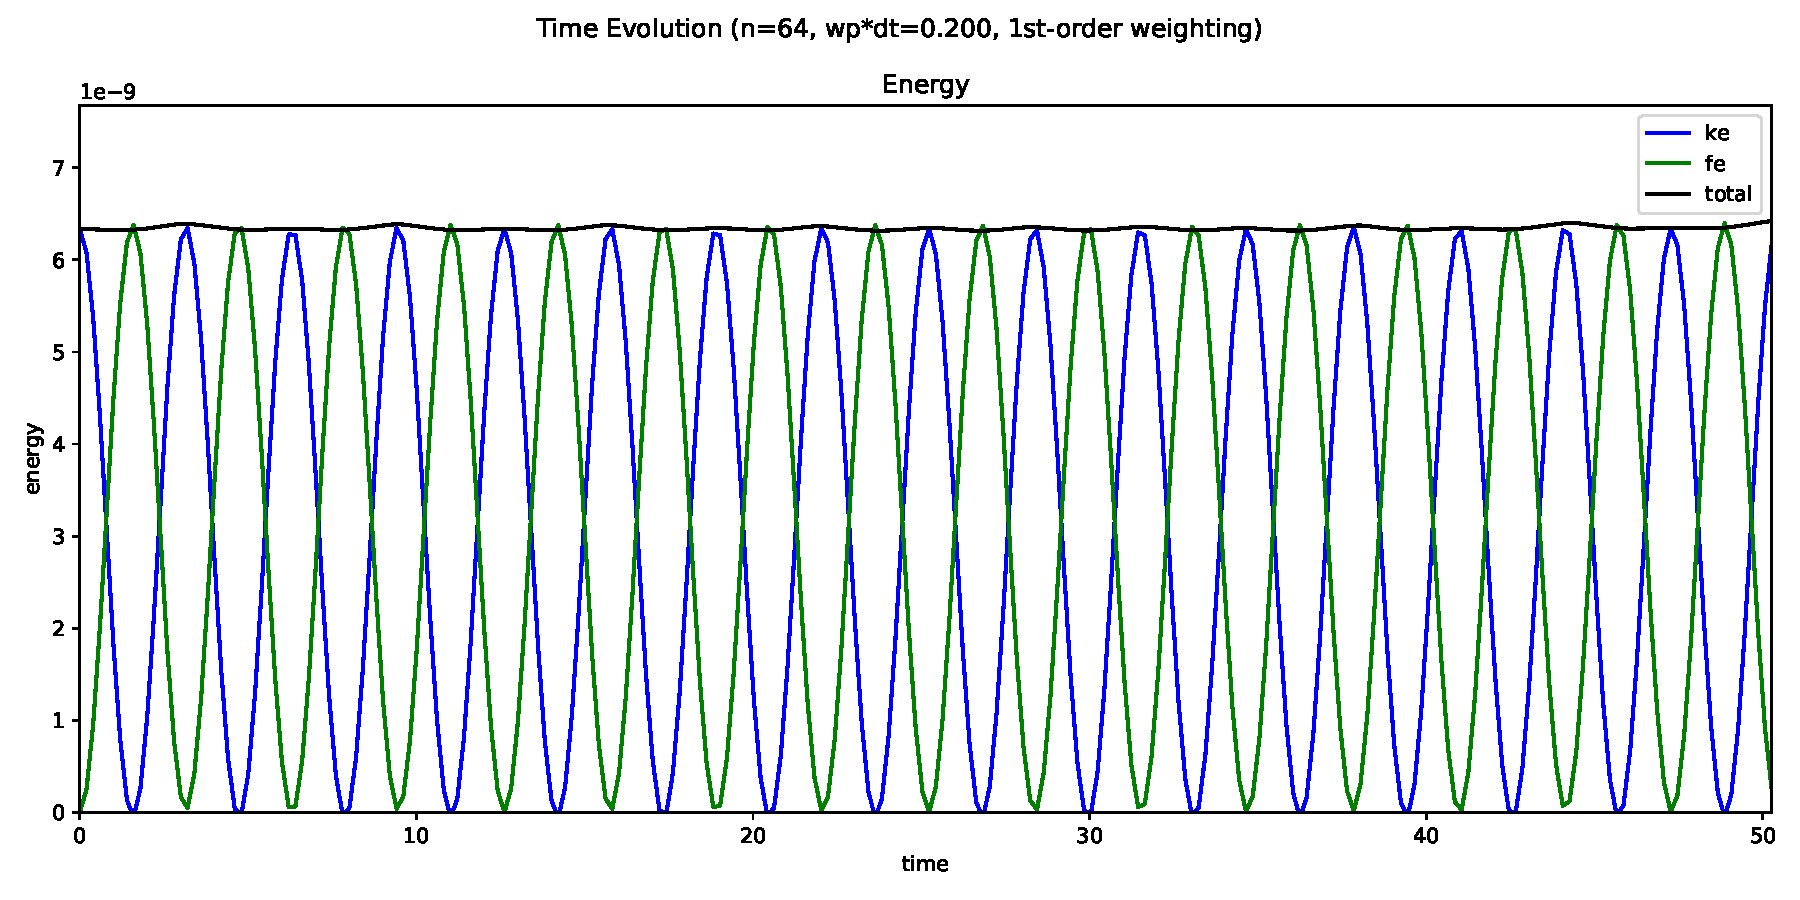
\includegraphics[width=0.9\linewidth]{proj2/leapfrog-stable.pdf}
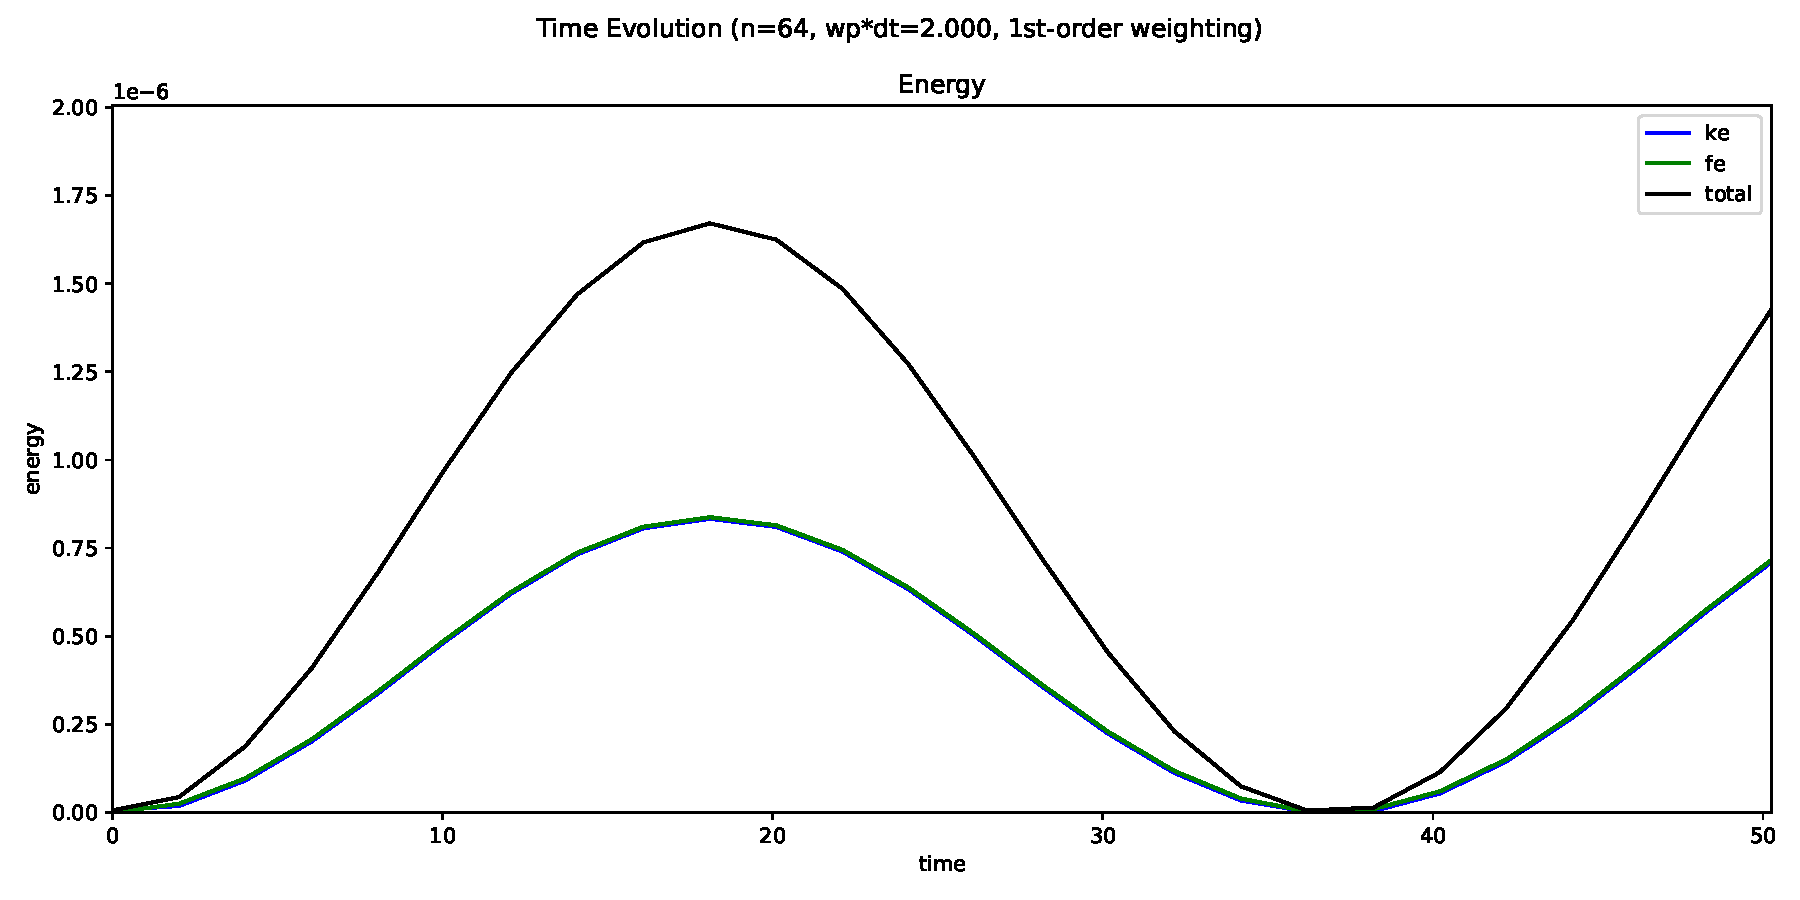
\includegraphics[width=0.9\linewidth]{proj2/leapfrog-unstable.pdf}
\caption{\label{fig:leapfrog-init}Leapfrog instability. As we increase $\Delta t$, the solution to the homogeneous finite difference equation becomes imaginary. At $\omega_p \Delta t / 2 = 0.2$, the sinusoidal perturbation maintains its frequency. At $\omega_p \Delta t = 2$, the solution explodes.}
\end{figure}

\begin{equation}
\frac{x^{t + \Delta t} - 2 x^t + x^{t - \Delta t}}{\Delta t^2} = - \omega_0 ^2 x^t
\end{equation}

Assuming a solution of the standard form $x^t = A e^{- i \omega t}$, we arrive at the dispersion relation

\begin{equation}
\sin \left( \omega \frac{\Delta t}{2} \right) = \pm \omega_0\frac{\Delta t}{2}
\end{equation}

At $\Delta t \omega_p \ll 2$, the dispersion is minimal and $\omega \approx \omega_p$. However, as we increase $\Delta t \omega_p$, the phase error grows. At $\Delta t \omega_p = 2$, the solution becomes complex, and we enter a region of numerical instability.

\nocite{*}

% \bibliography{proj1}% Produces the bibliography via BibTeX.

\end{document}
%
% ****** End of file apssamp.tex ******
